\section{The DOI Data Model}
\label{sec:DataModel}
In traditional eye-tracking analyses, AOIs are image sub-regions with particular semantic meaning. By analogy, DOIs are subsets of a visualization's underlying data. For example, in a network visualization, DOIs may be individual nodes or clusters of nodes. In a 3D scene-rendering they may be objects or components of objects that are part of the scene. When DOIs have corresponding visual representations in the visualization's output, then gaze coordinates can be mapped to DOIs via these representations. Bernhard et al.~\cite{bernhard2014gaze} and Alam et al.~\cite{alam15analyzing} describe practical ways in which DOIs can be defined and collected. The structure of DOI data is summarized in Figure~\ref{fig:dataModel}, describe in detail in the following paragraphs, and exemplified for concrete application domains in Table~\ref{tab:ExampleDOI}. 

A data visualization is designed and coded to support a specific data model, while instantiations of the visualization then turn datasets which conform to the model into visual output. A DOI instrumentation generally specifies how a data model should be partitioned into DOIs, while actual DOIs are ultimately created at run-time from specific data set instances. For example, we would define that each node in a network visualization should be a DOI, but node-DOIs get created at run-time from specific datasets shown by an instrumented visualization.

To further our discussion we will approximate a visualization's data model using the generic entity-attribute-value (EAV) data model~\cite{deran1991entity}, in which data entities are described by combinations of attribute-value pairs. More complex data models can be captured by extending the EAV paradigm to capture classes and relationships between entities (EAV/CR).  A specific instance of such a data model (i.e., a data set will contain a configuration of entities, attributes, values, and relationships that conform to the data model in Figure~\ref{fig:dataModel}, `data instance').  

DOIs are created as subsets of data instances, and are characterized by entities, attributes, and values contained in that subset Figure~\ref{fig:dataModel}, `DOI data subsets'). For example, DOIs could be defined for each node in a node-link visualization of interacting proteins, and described by the protein's attributes (e.g., label, type, function). However, DOIs could also be created for larger subsets of data, such as for example a meta-node in a hierarchical node-link visualization. In this case, the DOIs would encompass data from multiple entities. These options are captured in Figure~\ref{fig:dataModel}. Deciding how to assign data into DOIs depends on two factors: what the data models is, and which data subsets make sense as visual units in the instrumented visualization. 

A DOI instrumentation will report which DOIs users have viewed over time during each of their fixations (Figure~\ref{fig:dataModel}). Both Bernhard et al.~\cite{bernhard2014gaze} and Alam et al.~\cite{alam15analyzing} compute candidate objects a user is likely to have viewed during a fixation by considering not just the fixation point, but also a small area around it.  If multiple DOIs intersect that area, Bernhard et al. report only the object closest to the fixation, while Alam et al. report all viewing candidates.  The authors' arguments for these choices reduce to a discussion on whether users can focus on multiple objects concurrently and is not the focus of our paper. For a more general DOI data model we will simply consider Alam et al.'s approach. 

As such, each fixation may be associated with one viewed DOI, multiple viewed DOIs, or no viewed DOI. Moreover, our confidence that a DOI was indeed the locus of the user's attention is proportional to the proximity of the fixation to the DOI, and thus variable~\cite{alam15analyzing}. For example, in Figure~\ref{fig:dataModel}, we are less confident that the user viewed $DOI_2$ during their fifth fixation (taller DOI glyph), than we are that they viewed $DOI_1$ during their first (shorter DOI glyph). 

In a typical eye-tracking experiment DOI sequences would be captured for multiple users, and data describing those users (e.g., background, level of expertise, demographics) may also be collected. We do not capture this aspect in our data model but use it when we define our task taxonomy and visual design space. Similarly, our model is confined to DOI data and does not include information about the visual contexts in which each DOIs have been viewed.  While such information should be accessible in practice during an analysis, either as screen captures or reproducible visualization states, we felt that existing work thorough addresses eye-tracking analyses in stimulus space. 

Finally, we note that Bernhard et al. also provide a description of data that gaze-to-object mapping produces~\cite{bernhard2014gaze}. While defined exclusively in the context of 3D scene stimuli and somewhat less general, their description is fundamentally similar to ours and has informed the present exposition. 


\begin{figure}[!htb]
  \centering
  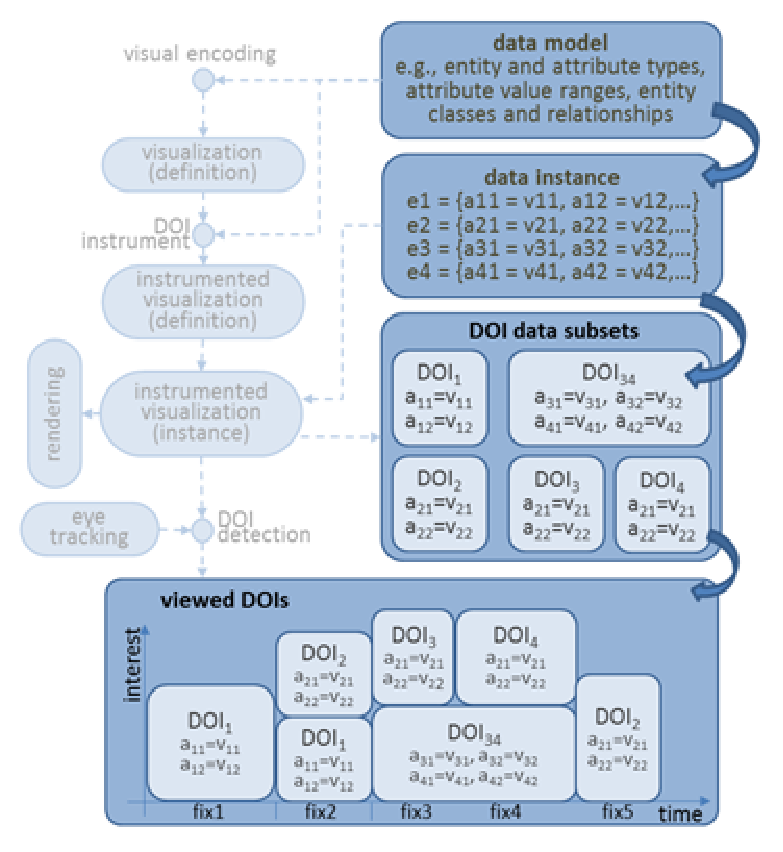
\includegraphics[width=\linewidth]{images/DOIDataModel.eps}
  \caption{DOI data model, DOI definition and collection. }
	\label{fig:dataModel}
\end{figure}

\begin{table*}[htbp]
	\centering
		\begin{tabular}{|l|l|l|}
			\hline
			\multicolumn{3}{|l|}
			{\shortstack[l]{
			\textbf{Data Model :}IMDB.org movie data shown as a PivotPaths diagrams~\cite{alam15analyzing}: movies, actors, genres, and directors are\\ displayed as glyphs and connected by links if they are related}
			}\\\hline
		 \shortstack[l]{\textbf{Data Instance :}\\
							$m_1=$\{type:`movie', label:`Dark Knight',rating:9\} \\
							$m_2=$\{type:`movie', label:`Big Fish', rating:7\}\\
							$a_1=$\{type:`actor', label:`Al Pacino', gender:`male'\}}
		& \shortstack[l]{\textbf{DOIs :}\\
									$DOI_1 = \{m_1\}$\\
									$DOI_2 = \{m_2\}$\\
									$DOI_3 = \{a_1\}$}
		&\shortstack[l]{\textbf{DOI Output :}\\
							$f_1=\{(DOI_1, 0.9),$\\$(DOI_2, 0.5)\}$\\
							$f_2 = \{(DOI_3,1.0)\}$}
		\\\hline
		\multicolumn{3}{|l|}
		{\textbf{Data Model :}	Learning content (e.g., architecture concepts) shown in a visual learning environment}\\\hline
		\shortstack[l]{\textbf{Data Instance :}\\
							$d_1=$\{type:`definition',format:`text', concept:`structure',level:`intro'\}\\
							$e_1=$\{type:`example',format:`image',concept:`structure',level:`intro'\}\\
							$f_1=$\{type:`formula', concept:`structure', level:`intro', partOf:$e_1$\}\\
							$l_1=$\{type:`legend', concept:`structure', level:`intro', partOf:$e_1$\}}					
		& \shortstack[l]{\textbf{DOIs :}\\
							$DOI_1 = \{d_1\}$\\
							$DOI_2 = \{e_1\}$\\
							$DOI_3 = \{f_1\}$\\
							$DOI_4 = \{l_1\}$
		}									
		&\shortstack[l]{\textbf{DOI Output :}\\
							$f_1 = \{(DOI_1,0.8)\}$\\
							$f_2=\{(DOI_2, 1),$\\$(DOI_3, 0.8)\}$\\
							$f_3=\{(DOI_2, 1),$\\$(DOI_3, 0.7)\}$
							}
		\\\hline
		\multicolumn{3}{|l|}
		{\textbf{Data Model :}A 3D scene (e.g., a construction scene used in studying construction-safety designs)}\\\hline
		 \shortstack[l]{\textbf{Data Instance :}\\
							$w_1=$\{type:`worker',helmet:yes,vest:yes,boots:yes\}\\
							$w_2=$\{type:`worker',helmet:no,vest:yes,boots:yes\}\\
							$m_1 =$ \{type:`material',category:`concrete\_block'\}\\						
							$o_1 =$ \{type:`machinery',category:`crane',load:$m_1$\}\\
							$o_2 =$ \{type:`machinery',category:`bulldozer'\}
							}
		& \shortstack[l]{\textbf{DOIs :}
							$DOI_1 = \{w_1\}$\\
							$DOI_2 = \{w_2\}$\\
							$DOI_3 = \{w_1, w_2\}$\\
							$DOI_4 = \{m_1\}$\\
							$DOI_5 = \{o_1\}$\\
							$DOI_6 = \{o_2\}$\\
							$DOI_7 = \{o_1,o_2\}$
		}									
		&\shortstack[l]{\textbf{DOI Output :}\\
							$f_1 = \{(DOI_2,0.75)\}$\\
							$f_2 = \{(DOI_3,0.9)\}$\\
							$f_3=\{(DOI_5, 0.9),$\\$(DOI_4, 0.7)\}$\\
							$f_3=\{(DOI_7, 1),$\\$(DOI_4, 0.65)\}$
							}
		\\\hline
		\end{tabular}
		\caption{Examples of DOIs.}
		\label{tab:ExampleDOI}
\end{table*} 

\subsection{AOI vs DOI}
\label{sec:AOIvDOI}
There are significant differences between AOIs and DOIs. Describing them helps clarify the properties of DOI data and motivates the need for new research in DOI analysis.

\textbf{\underline{Data collection :}} AOIs exist in stimulus or image space, and need to be defined for each visual frame a user sees. AOI analyses can be used for any type of visual stimulus and drawing AOIs onto images requires little expertise. 

Instead, DOIs are defined over a visualization's underlying data by instrumenting the visualization's code. Once a visualization instrumented, DOI data can be collected without additional effort for any new dataset that the visualization can show. Moreover, because DOIs are defined over data, their collection is immune to a subject's interactions with a system and specific views they create. This means that data can be captured easily from interactive systems over extended periods of time~\cite{alam15analyzing}. On the downside, the code of the visualization needs to be open and analysts need to have the expertise to instrument it.

\textbf{\underline{Data scale and granularity :}} AOIs tend to be large and sparse (e.g., an entire view or interface panel), and analyses often involve few AOIs. Moreover, AOI analyses tend to be limited to static stimuli or short videos since defining AOIs over many stimulus frames is costly. Conversely, DOIs can be granular and many (e.g., individual objects). Because data collection doesn't involve manual annotation, DOI data can be collected over long periods of time. As such, DOI analyses can involve hundreds of DOIs and thousands of focus switches between them. Moreover, DOIs can be defined hierarchically or in groups. 

\textbf{\uline{Attributes :}} AOIs have implicit properties known to the analyst but generally not expressed explicitly (e.g., the type or role of an AOI). Instead, DOIs have explicit semantic attributes that are automatically derived from a visualization's data. 

\textbf{\underline{DOI data is probabilistic :}} AOIs are generally large, broadly defined, and do not overlap. As such, users often fixate within one particular AOI. Instead, DOIs can be small and close together. Viewers may fixate in the vicinity of multiple DOIs, and often fixate close but not necessarily on any particular DOI. DOI detection is therefore probabilistic: we detect a likelihood that an object is viewed during a fixation rather than a certainty. Moreover, multiple objects may be viewed at the same time.

\textbf{\underline{Questions they can answer :}} AOI analyses generally explore key-hole scenarios involving static stimuli, constraint interactions, or short videos. They are aimed at exploring perceptual processes and often support the testing of well bounded hypotheses. Instead, DOI analyses can be applied to study the use of interactive visual interfaces ``in vivo''. It can answer questions about which data users are interested in, and how they might use this data to reason and hypothesize, and is less apt for studying visual perception. Through its scale and semantic annotation, DOI data supports data driven, exploratory analyses. 
 










